% position image in center
\begin{figure}[h]
    \centering
    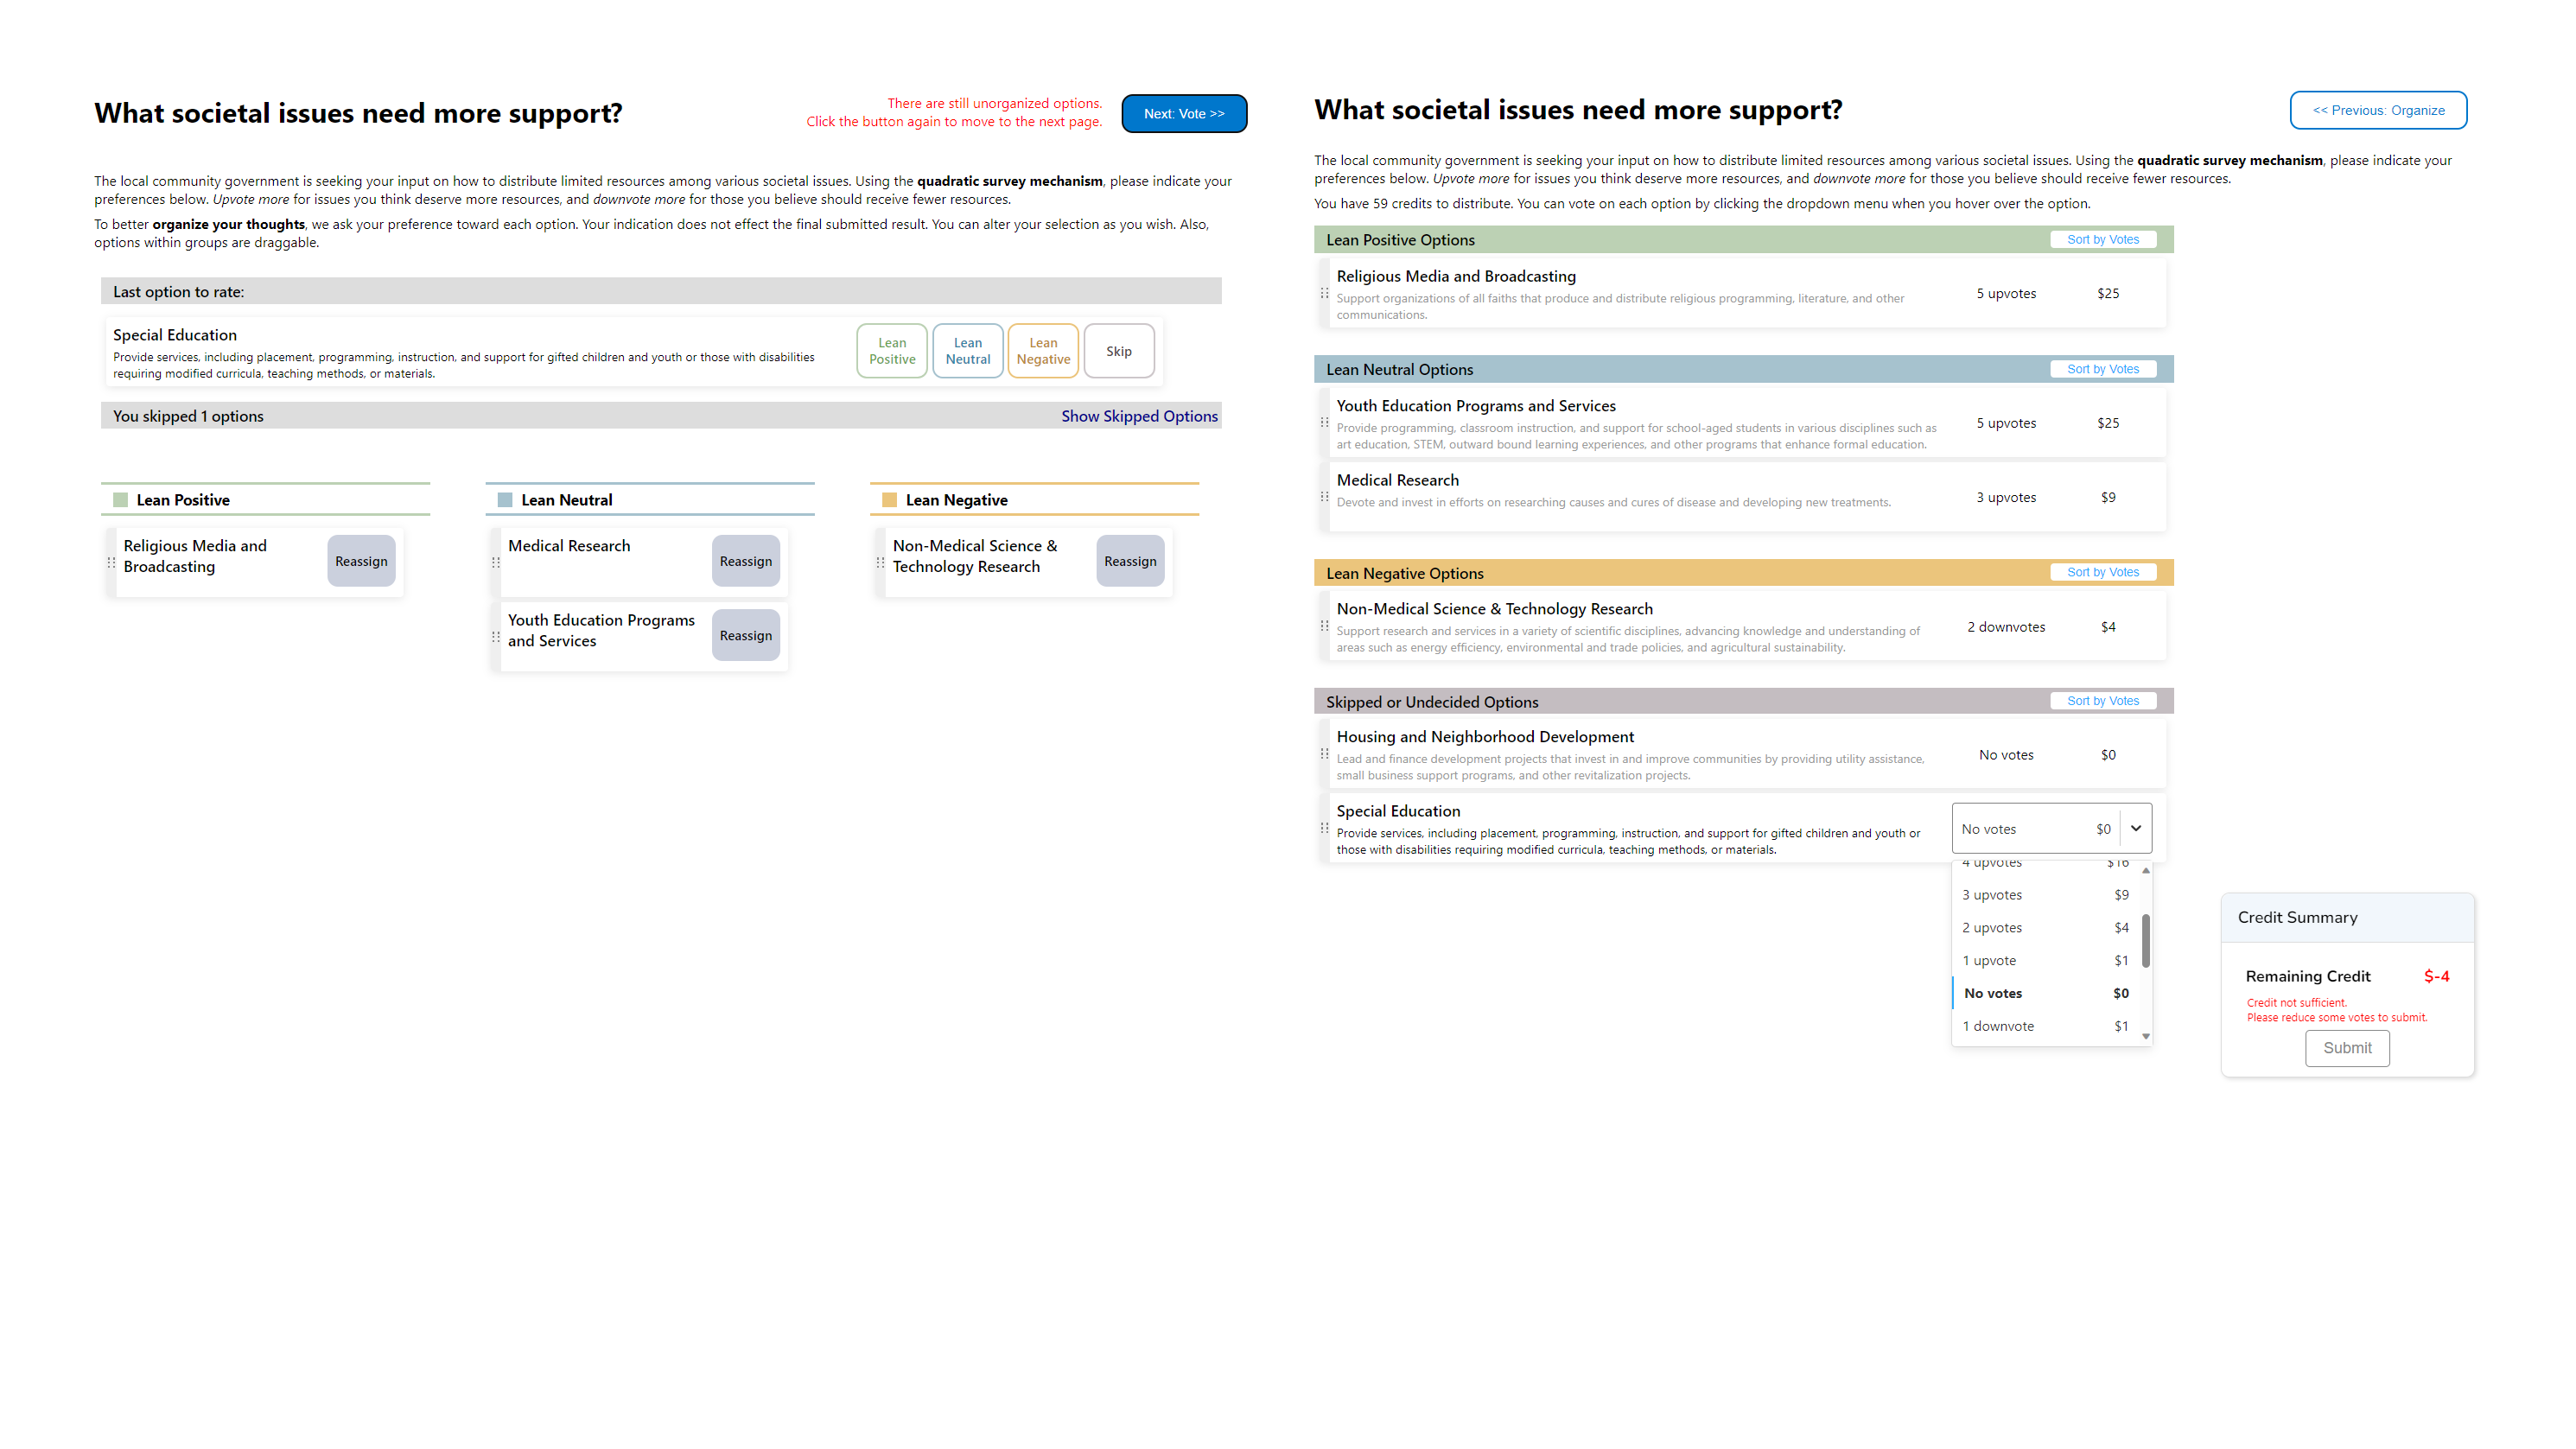
\includegraphics[width=1\textwidth]{content/image/interface.png}
    \caption{The interactive interface}
    \label{fig:interactiveInterface}
\end{figure}

\section{Experiment Design}
To answer our research question, we developed an open-source system with a interface specifcially for quadratic surveys. We then designed a two-by-two, mixed method experiment to examine how number of options and the interface type affect the participants. This section detail each experiment component.

\subsection {System Design}
We designed an interactive text interface (ITI) and a baseline text interface (BTI) for this study. We begin from describing BTI. In order to better understand the influence of number of options and different interface components to support QS, we identified essental components for QS (detailed deliberation in appendix.). Different from many prior research (cite several paper here), we intentially removed all data visualization elements as inappropriate visualizations might increase mental demand (huangMeasuringEffectivenessGraph2009) rather then reduce the demand. Thus, in the BTI interface (figure X), participants are presented with a list of options with a system prompt on top. Each option has a dropdown that provides all possible voting options and cost given the number of credits. A small summary box is to the right of the interface showing the current cost and the remaining credit.

The ITI interface (figure Y) builds on top of the BTI interface with two additional components. The first acts as a scaffolding process of supporting individuals responds to QS given its complexity. This mainly focuses on breaking QS into two steps -- first organizing thoughts and then vote -- to provide respondents with a structured way to express their preferences. On organizing the options (figure Y-a), respondents are shown 


ranking and then voting -- hoping  In the first step, invidiuals are shown all options on the survey one at a time, prompting to `categorize' options into three ordinal categories. Participants are aware that they can choose not to rank the options at all

We utilize a drag-and-drop direct manipulable interface to nudge individuals to sort the options (see Figure \ref{fig:rank}), then we ask individuals to vote based on the sorted list. We hypothesize that the sorting step forces participants to think only about the ranks and not the degree of preference. With an (almost) sorted list, individuals can limit their working memory to only consider the strength of preferences among the options above or below an option. In addition, if the participants do not want to sort the options, the drag-and-drop functionality can also act as a way to organize the options' proximity freely. For example, participants can cluster the options toward the top, middle, or bottom of the list to represent three sets of responses they want to express. Again, such a design aims to reduce the cognitive burden of remembering and keeping track of all options. 

The notion of drag-and-drop has been explored widely in rank-based surveys. For instance, \textcite{krosnick2018measurement} demonstrated that replacing drag-and-drop with traditional number-filling rank-based questions improved participants' satisfaction with a little trade-off in their time. A similar work embedded drag-and-drop as part of its ranking process~\cite{timbrook2013comparison}. Since the rank-then-vote rationale asks participants first to rank and vote, we adopt such a design. Additional justification would be added in later versions.



In our study, we developed a software interface consisting of a two-step process to facilitate participant interaction with quadratic surveys. Initially, participants are introduced to the first step, where they are invited to organize their thoughts using a three-point Likert scale that includes a no-response option. This feature allows for an initial subjective categorization, empowering participants to define their own criteria for assessment. Following this, the system presents the results by grouping the options, which participants can adjust to their preference at any point, thus offering a tailored review process.

Moving to the second step, the interface seamlessly transitions to the standard Quadratic Survey (QS). Here, the options previously organized are displayed, maintaining the order from the first step to provide continuity. Participants engage with the QS by utilizing a drag and drop feature, which was chosen based on findings from Duncan Rintoul's 2019 study that suggested such an interface is subjectively preferred, despite lower stability. This design decision prioritizes user experience, emphasizing the importance of interface affability and ease of use.

The entire interface is displayed on a vertically oriented 32-inch monitor, the largest available at the time, to eliminate the need for scrolling. This decision was made to minimize cognitive load, a primary goal of our interface design, especially crucial when participants are presented with lengthy options. Our aim is to present all available choices concurrently to reduce the extra cognitive effort that scrolling could impose.

To enhance the usability and understandability of our interface, we conducted multiple iterations of pilot testing. These tests were instrumental in refining the design, leading to a minimalistic approach that strips away non-essential visual elements such as data visualizations, icons, and images. This design philosophy, which is detailed in the Appendix, aligns with our goal of minimizing cognitive load and ensuring that participants can focus solely on the survey content.

Through this meticulously designed interface, we aim to reduce the decision space for participants, encouraging thoughtful engagement and deliberate choice without overwhelming them. By allowing participants to rank before rating, we facilitate a decision-making process that discourages mental shortcuts and promotes a more reflective, System 2 type of thinking. The adjustments made as a result of our pilot studies have been crucial in achieving an interface that supports our research objectives while also being intuitively navigable by our participants.

Participants initially engage with the interface using a three-point Likert scale for subjective categorization. This step allows participants to define their own assessment criteria, empowering them for a tailored review process.

\subsection{Second Step}
The interface transitions to the standard Quadratic Survey (QS), displaying the options organized in the first step. A drag and drop feature is used for engaging with the QS, enhancing user experience based on findings from Duncan Rintoul's 2019 study.

\section{Enhancing Usability and Minimizing Cognitive Load}
To minimize cognitive load and enhance usability, the interface is displayed on a 32-inch vertical monitor. This setup prevents the need for scrolling and allows all options to be presented concurrently. Multiple iterations of pilot testing led to a minimalistic design, stripping away non-essential visual elements.

\section{Rationale Behind Experimental Design}
A two-by-two experiment was designed to evaluate the interface, involving varying numbers of options and interface types.

\subsection{Experiment Flow and Participant Grouping}
\begin{itemize}
    \item Participants are assigned to one of four groups, with different combinations of options and interface types.
    \item The experiment flow includes consent form signing, QS instructions, a QS understanding quiz, and completing surveys using the interfaces, followed by cognitive load and motivation questionnaires.
\end{itemize}

\section{Justification for Key Methodological Choices}
\subsection{Why In-Person}
The in-person nature of the experiment is crucial for controlling environmental variables and accurately measuring cognitive load. This setup also allows for capturing individual behaviors without the need for additional software.

\subsection{Between-Subject Design}
A between-subject design is chosen over a within-subject design to reduce complexity and participant fatigue. This approach also helps to control for learning effects and dropout rates.

\subsection{Interface Design Considerations}
The interface design includes the Rank-then-Vote and Tag-then-Vote approaches, aimed at providing a structured way for preference expression and reducing cognitive burden.

\section{Selecting the Number of Options}
The decision to use 6 and 24 options is based on literature recommendations and experiments designed for choice overload. This choice is aligned with the goal of understanding the impact of option number on cognitive load.

\section{Evaluation Methods}
\subsection{Cognitive Load}
Cognitive load is measured using NASA-TLX, a subjective tool widely used in the HCI community. This method is chosen for its simplicity and effectiveness in capturing cognitive load in longer tasks like QS.

\subsection{Participant Motivations}
Participant motivations are assessed using SIMS (Situational Motivation Scale), which measures motivation based on four types: intrinsic, identified regulation, and external regulation. The scale's application is aligned with understanding why individuals engage in the activity.


\section{System Design}



\section{Experiment and Interface Design}


In this section we will first describe our interface design, followed by the experiment design.
\subsubsection{}
Mentioned the importnace of stripping away visualization to test the core mechanism of QV.
inspired by news article on surface area, but stress people's difficulty in understanding the concept of surface area and diffing them





Workload experience is a constructive cognitive process that combines immediate experiences and preconceptions. 
It is difficult to evaluate as the attributes that contribute to the workload experience vary between different tasks and evaluators. Currently, there are a few popular evaluation methods, including performance measures, psychophysiological measures, subjective measures, and analytical measures. [1] It is hard to adopt the performance measures such as secondary-task measures in our experiment since it is hard to design the secondary task. The secondary task requires to use of the same cognitive resources as the primary tasks, and the cognitive resource for filling in the survey would be variable depending on different participants. [2] Subjective measures use self-report ratings to collect options from participants. [3] Although there is criticism about its validity and vulnerability, it is the most commonly used measurement because of its low cost and ease of administration.  Because of these considerations, our study would focus on subjective measures.[1] NASA Task Load Index (TLX) is one of the most widely used subjective measures. It is a multidimensional scoring procedure that uses the weighted average of six subscale scores to represent the overall workload. The six subscales include the dimensions related to the demands imposed on the subject (mental demands, physical demands, and temporal demands) and the interaction of a subject with the task (performance, effort, and frustration). [4][5][6] NASA-TLX uses a priori workload definition of subjects to weight and average subscale ratings, which asks the subject to evaluate the contribution of each weight to the workload of a specific task. [4] This process would decrease the between rater variability since it indicates the differences in workload definition between raters within a task and the differences in the sources of workload between tasks. [6][7] It provides diagnostic information on the nature of the workload associated with the task. In addition, the NASA-TLX rating scales represent comparative judgments concerning extreme values with natural psychological significance.[8] In addition, its grading scales include 21 gradations, which help NASA-TLX considerably decrease its sensitivity and increase its variability between subjects compared with other subjective measures like SWAT which has only three discrete values. [9] NASA-TLX has been tested on a variety of experimental tasks and lab tasks, and the workload scores derived from these tests were found to have significantly less variability of the evaluators than the one-dimensional workload scores. Based on the above reasons, we would use NASA-TLX to measure the cognitive load in our study.
\smallskip
\newline Reference:
\newline [1] \href{https://www.tandfonline.com/doi/full/10.1080/00140139.2013.790483}{Using GOMS and NASA-TLX to Evaluate Human–Computer Interaction Process in Interactive Segmentation} 
\newline [2] \href{https://link.springer.com/content/pdf/10.1007/978-1-4757-0884-4.pdf}{Mental Workload:Its Theory and Measurement}
\newline [3] \href{https://www.cambridge.org/core/services/aop-cambridge-core/content/view/8B34A19A05BC442D9AB5F17B637B16BF/9780511844744c9_p181-202_CBO.pdf/measuring-cognitive-load.pdf}{Measuring Cognitive Load}
\newline [4] \href{http://usd-apps.usd.edu/coglab/schieber/psyc792/workload/Hart-Staveland-1988.pdf}{Development of NASA-TLX (Task Load Index): Results of Empirical and Theoretical Research}
\newline [5] \href{https://journals-sagepub-com.proxy2.library.illinois.edu/doi/pdf/10.1177/154193120605000909}{NASA-TASK LOAD INDEX (NASA-TLX); 20 YEARS LATER}
\newline [6] \href{https://apps.dtic.mil/sti/citations/ADA474193}{A Review of the Mental Workload Literature}
\newline [7] \href{https://www.tandfonline.com/doi/10.1080/00140139.2010.489960}{Sensitivity and diagnosticity of NASA-TLX and simplified SWAT to assess the mental workload associated with operating an agricultural sprayer}
\newline [8] \href{https://www.sciencedirect.com/science/article/pii/S0166411508623869?via\%3Dihub}{Development of NASA-TLX (Task Load Index): Results of Empirical and Theoretical Research}
\newline [9] \href{https://iaap-journals.onlinelibrary.wiley.com/doi/full/10.1111/j.1464-0597.2004.00161.x?casa_token=NXvVjc_MTe0AAAAA\%3AtQY52tj5cDyCZSJBwAv8uDUCu9WYOVFOckHK7TuHG1DExG639DE_ayjtnNrIWyBezv9l1T-odSevaxo}{Evaluation  of  Subjective  Mental  Workload:  A  Comparison  of  SWAT,  NASA-TLX,  and  Workload  Profile  Methods}